\section{System Description}
\subsection{Hybrid Systems}

Let $H = \langle X, Q, \mathsf{flow}, \mathsf{jump},
\mathsf{inv},\mathsf{init}\rangle$ be a hybrid system, where
$\mathsf{flow}$, $\mathsf{jump}$, $\mathsf{inv}$, $\mathsf{init}$ are
SMT formulas that \texttt{dReal} can handle (first-order formulas over
the reals that allow polynomials, trigonometric functions, exponential
functions, Lipschitz-continuous ODEs, etc.)

Now specify a numerical error bound $\delta$, and recall that for any
formula $\varphi$ we have defined a notion of $\delta$-perturbation of
$\varphi$, written as $\varphi^{\delta}$. We can then define the
$\delta$-perturbation of $H$ as:

\[
H^{\delta} = \langle X, Q, {\mathsf{flow}}^{\delta},
{\mathsf{jump}}^{\delta}, {\mathsf{inv}}^{\delta},
{\mathsf{init}}^{\delta}\rangle,
\]

by simply relaxing the logic formulas in the representation of $H$.
Choose $n\in\mathbb{N}$ to be a bound on the number of discrete mode
changes and $T\in \mathbb{R}^+$ an upper bound on the time duration.
Let $\mathsf{unsafe}$ encode a subset of $X\times Q$, the state space
of $H$. The bounded $\delta$-reachability problem asks for one of the
following answers:

\begin{itemize}
\item  safe: $H$ cannot reach $\mathsf{unsafe}$ in $n$ steps within
  time $T$.
\item $\delta$-unsafe: $H^{\delta}$ can reach ${\mathsf{unsafe}}^{\delta}$ in $n$ steps within time $T$.
\end{itemize}

\subsection{drh: A Language for Hybrid Systems}
\begin{figure}
  \centering
  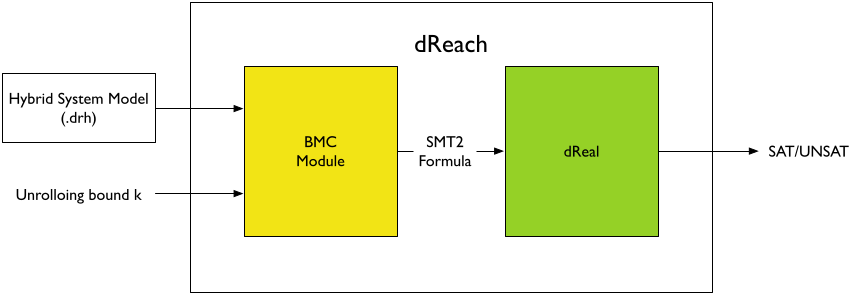
\includegraphics[width=\textwidth]{images/dReach}
  \caption{System Description}
  \label{fig:system-description}
\end{figure}

% 1. Define the input language (drh)
% 2. A small example of translation to logic formulas. Use two boxes,
% one drh, one smt2.

Example:

\begin{Verbatim}[fontfamily=courier, frame=single, framesep=5mm, numbers=left, fontsize=\footnotesize]
#define D 0.45
#define K 0.9
[0, 15] x;
[9.8] g;
[-18, 18] v;
[0, 3] time;

{ mode 1;

  invt:
        (v <= 0);
        (x >= 0);
  flow:
        d/dt[x] = v;
        d/dt[v] = -g + (- D * v ^ 1);
  jump:
        (x = 0) ==> @2 (and (x' = x) (v' = - K * v));
}
{
  mode 2;
  invt:
        (v >= 0);
        (x >= 0);
  flow:
        d/dt[x] = v;
        d/dt[v] = -g + (- D * v ^ 1);
  jump:
        (v = 0) ==> @1 (and (x' = x) (v' = v));
}
init:
@1    (and (x >= 5) (v = 0));

goal:
@1    (and (x >= 0.45));
\end{Verbatim}


%%% Local Variables:
%%% mode: latex
%%% TeX-master: "main"
%%% End:
